\subsection{题目描述}
\noindent Write a code to numerically solve the radial Schrödinger equation for
\[
\left[-\frac{1}{2}\nabla^2+V(\mathbf{r})\right]\psi(\mathbf{r})=E\psi(\mathbf{r}), \quad V(\mathbf{r})=V(r)
\]
\begin{enumerate}
    \item \( V(r) = \frac{1}{r} \) (hydrogen atom)
    \item Considering the following potential:
    \[
    V(r) = -\frac{Z_{\text{ion}}}{r}\text{erf}\left(\frac{r}{\sqrt{2} r_{\text{loc}}}\right) 
    + \exp \left[ -\frac{1}{2} \left(\frac{r}{r_{\text{loc}}}\right)^{2}\right]
    \times \left[C_1 + C_2\left(\frac{r}{r_{\text{loc}}}\right)^2+C_3\left(\frac{r}{r_{\text{loc}}}\right)^4+C_4\left(\frac{r}{r_{\text{loc}}}\right)^6\right]
    \]
\end{enumerate}
where \(\text{erf}\) is the error function. And for Li, you could set:
\begin{itemize}
    \item \( Z_{\text{ion}}=3 \)
    \item \( r_{\text{loc}}=0.4 \)
    \item \( C_1=-14.0093922 \)
    \item \( C_2=9.5099073 \)
    \item \( C_3=-1.7532723 \)
    \item \( C_4=0.0834586 \)
\end{itemize}
\noindent Compute and plot the first three eigenstates. You could find more information about 'how to solve radial Schrödinger equation' and 'use of non-uniform grid (optional)' in the PPT.

\textbf{Special Note:} You may call any library functions for diagonalization.


\subsection{程序描述}
本程序拥有四个模块:\texttt{utils},\texttt{solver},\texttt{analysis},\texttt{visualization},分别为工具函数和配置参数模块、数值求解算法模块、结果分析和处理模块与可视化处理模块。主程序入口\texttt{main}中有主求解器类\texttt{RadialSchrodingerSolver},其计算配置与非均匀网格由\texttt{utils}中的\texttt{SolverConfig}类与\texttt{RadialGrid}类指定;势能函数调用\texttt{utils}中的\texttt{Potential}基类,其中有本题设定的氢原子库仑势与锂原子局域势,\texttt{utils}中还有一些辅助工具,在此不一一列举。主求解器的核心逻辑依赖绑定的求解器实例\texttt{ShootingSolver}或\texttt{FiniteDifferenceSolver}\footnote{Numerov实在没时间写了qwq}.主求解器还从\texttt{analysis}模块绑定了波函数处理器\texttt{WavefunctionProcessor},负责计算导数、分析波函数渐进行为、根据不同角量子数由邻域外推原点附近的波函数奇异值、归一化处理等;能量分析器\texttt{EnergyAnalyzer},负责比较能级与理论值差异;收敛性分析器\texttt{ConvergenceAnalyzer},负责分析不同网格下的收敛性。最后,来自可视化模块\texttt{visualization}中的\texttt{ResultVisualizer}负责波函数、概率密度与收敛分析结果的可视化。
\subsection{伪代码}
Powered by \href{https://chatgpt.com/g/g-xJJAA2awf-latex-pseudocode-generator}{\LaTeX \ pseudocode generator}


\subsection{结果示例}
\subsubsection{打靶法计算结果}
\begin{threeparttable}
    \begin{tabular}{|c|c|c|c|c|c|}
    \hline
    原子 & 量子数 \(n, l\) & 能级 (单位: hartree) & 原子 & 量子数 \(n, l\) & 能级 (单位: hartree) \\ \hline
    \multirow{6}{*}{氢原子} & \(n=1, l=0, 1s\) & -0.500000 & \multirow{6}{*}{锂原子} & \(n=1, l=0, 1s\) & -4.458247 \\ \cline{2-3} \cline{5-6}
                            & \(n=2, l=0, 2s\) & -0.125000 &                      & \(n=2, l=0, 2s\) & -1.115432 \\ \cline{2-3} \cline{5-6}
                            & \(n=2, l=1, 2p\) & -0.125000 &                      & \(n=2, l=1, 2p\) & -1.122278 \\ \cline{2-3} \cline{5-6}
                            & \(n=3, l=0, 3s\) & -0.055556 &                      & \(n=3, l=0, 3s\) & -0.496256\tnote{b} \\ \cline{2-3} \cline{5-6}
                            & \(n=3, l=1, 3p\) & -0.055556\tnote{a} &                      & \(n=3, l=1, 3p\) & -0.498679 \\ \cline{2-3} \cline{5-6}
                            & \(n=3, l=2, 3d\) & -0.055556 &                      & \(n=3, l=2, 3d\) & -0.500262 \\ \hline
    \end{tabular}
    \begin{tablenotes}
        \item[a] 对于 \(n=3\) 的三个态,指定了 \texttt{r\_Max=60},精度大幅提高,但下面图片为展现边界效应未替换

    \item[b] 对于 \(n=3\) 的三个态,指定了 \texttt{r\_Max=60},否则无法收敛,甚至边界发散
    \end{tablenotes}
    \end{threeparttable}
    \subsubsection{有限差分法计算结果}
    \begin{threeparttable}
        \begin{tabular}{|c|c|c|c|c|c|}
        \hline
        原子 & 量子数 \(n, l\) & 能级 (单位: hartree) & 原子 & 量子数 \(n, l\) & 能级 (单位: hartree) \\ \hline
        \multirow{6}{*}{氢原子} & \(n=1, l=0, 1s\) & -0.499993 & \multirow{6}{*}{锂原子} & \(n=1, l=0, 1s\) & -4.458266\tnote{d} \\ \cline{2-3} \cline{5-6}
                                & \(n=2, l=0, 2s\) & -0.125007 &                      & \(n=2, l=0, 2s\) & -1.115469 \\ \cline{2-3} \cline{5-6}
                                & \(n=2, l=1, 2p\) & -0.125003 &                      & \(n=2, l=1, 2p\) & -1.122296 \\ \cline{2-3} \cline{5-6}
                                & \(n=3, l=0, 3s\) & -0.055556\tnote{a} &                      & \(n=3, l=0, 3s\) & -0.496337 \\ \cline{2-3} \cline{5-6}
                                & \(n=3, l=1, 3p\) & -0.031255\tnote{b} &                      & \(n=3, l=1, 3p\) & -0.280662\tnote{e} \\ \cline{2-3} \cline{5-6}
                                & \(n=3, l=2, 3d\) & -0.055529\tnote{c}&                      & \(n=3, l=2, 3d\) & -0.500269\tnote{f} \\ \hline
        \end{tabular}
        \begin{tablenotes}
        \item[a] 在\texttt{r\_Max=30}偏差过大,提升至60
        \item[b] 实际上是4p态,但始终找不到正确的3p,可能是窗口设置太小
        \item[c] 3d态在\texttt{r\_Max=30}表现尚好,因其极大值离核,边界效应不显著
        \item[d] 使用\texttt{r\_Max=30},\texttt{j\_Max=300},表现良好 
        \item[e] 实际上应该是4p态,但也始终找不到正确的3p
        \item[f] 提升至\texttt{j\_Max=400}后与打靶法结果差距更小
        \end{tablenotes}
        \end{threeparttable}

\subsubsection{输入与异常处理}
\begin{figure}[H]
    \centering
    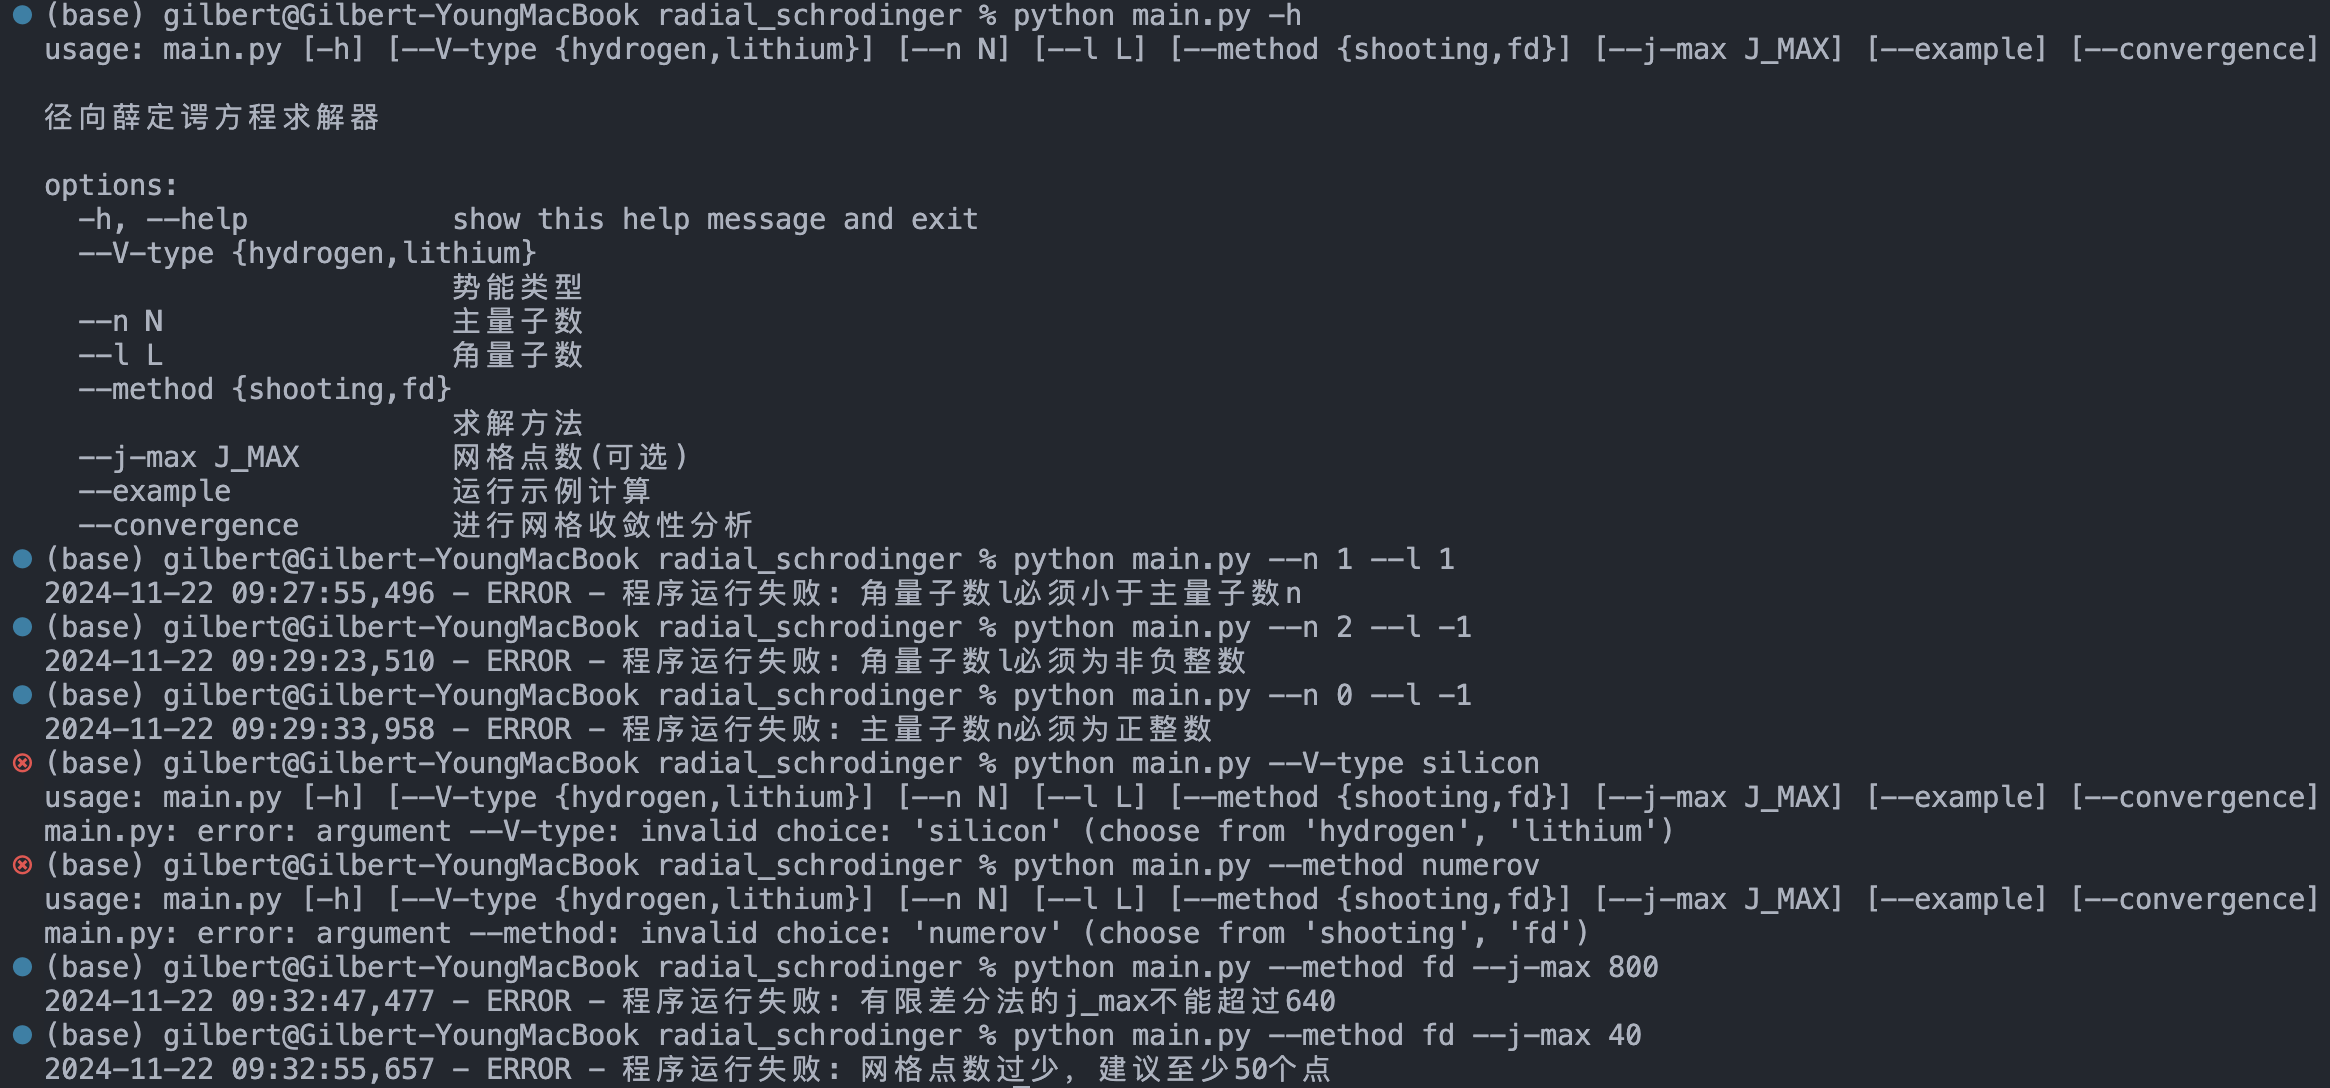
\includegraphics[width=1.0\textwidth]{Problem_2/figs/error-terminal.png}
    \caption{自定义参数输入与异常处理,新版本支持网格起止点\texttt{r\_min}与\texttt{r\_Max}的指定}
\end{figure}

\subsubsection{使用example选项运行的示例}
\begin{figure}[H]
    \centering
    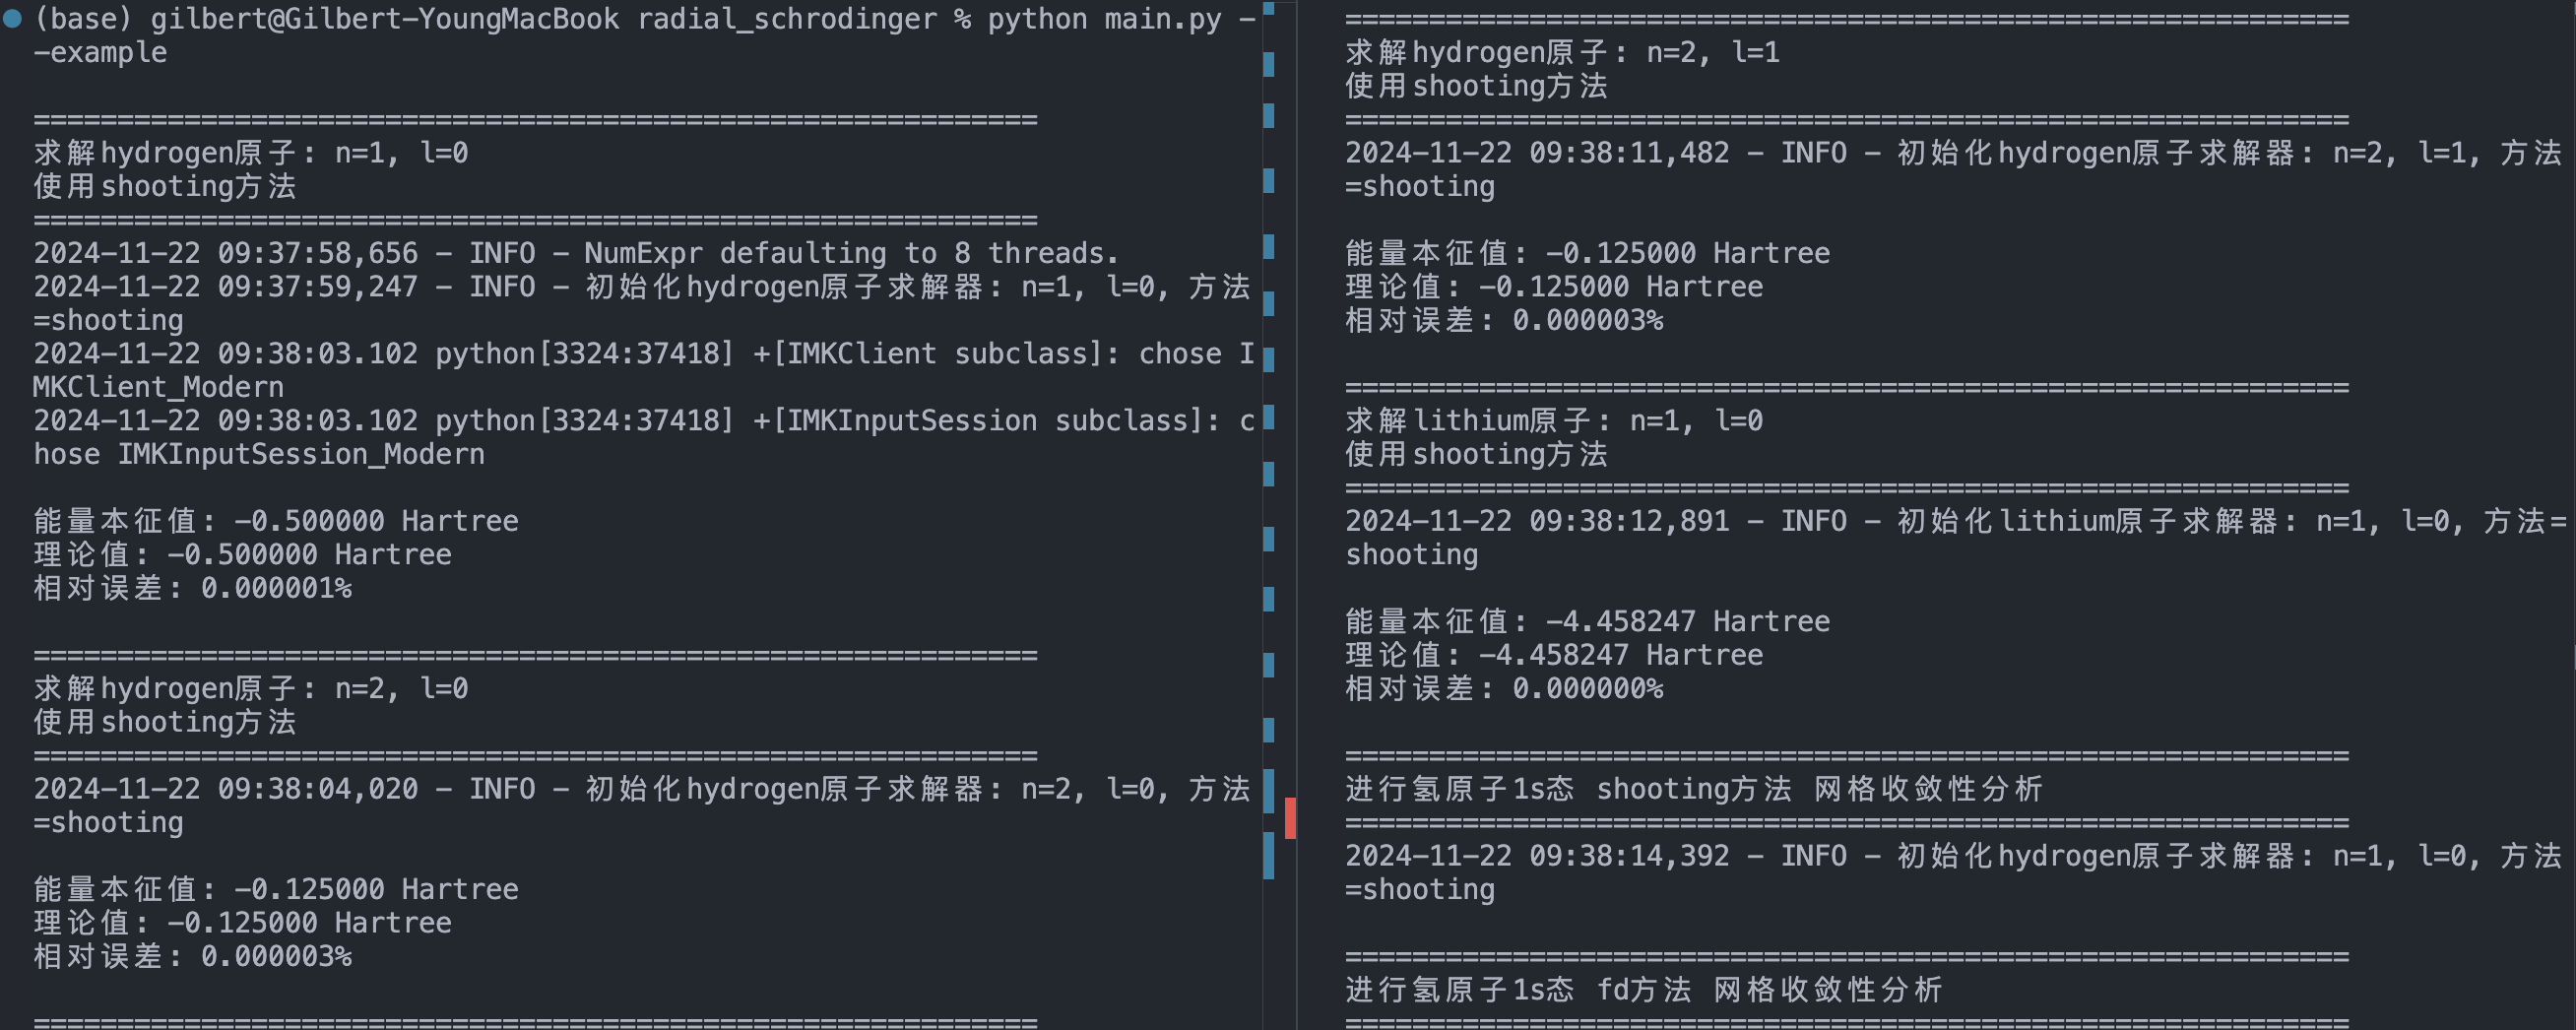
\includegraphics[width=1.0\textwidth]{Problem_2/figs/example-terminal.png}
    \caption{运行示例的终端输出}
\end{figure}

\begin{figure}[H]
    \centering
    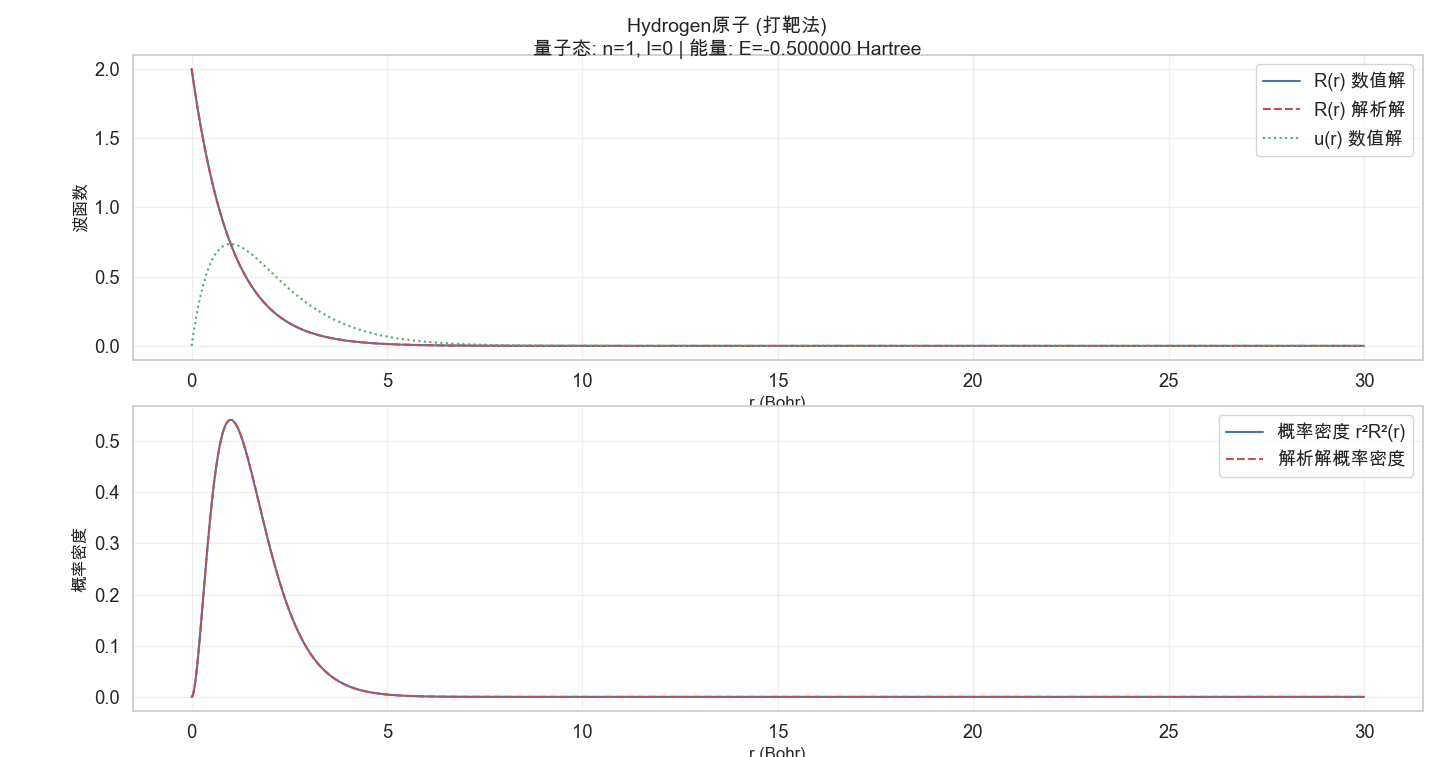
\includegraphics[width=1.0\textwidth]{Problem_2/figs/example_h_shooting_1s.png}
    \caption{使用打靶法求解氢原子库仑势的1s态}
\end{figure}

\begin{figure}[H]
    \centering
    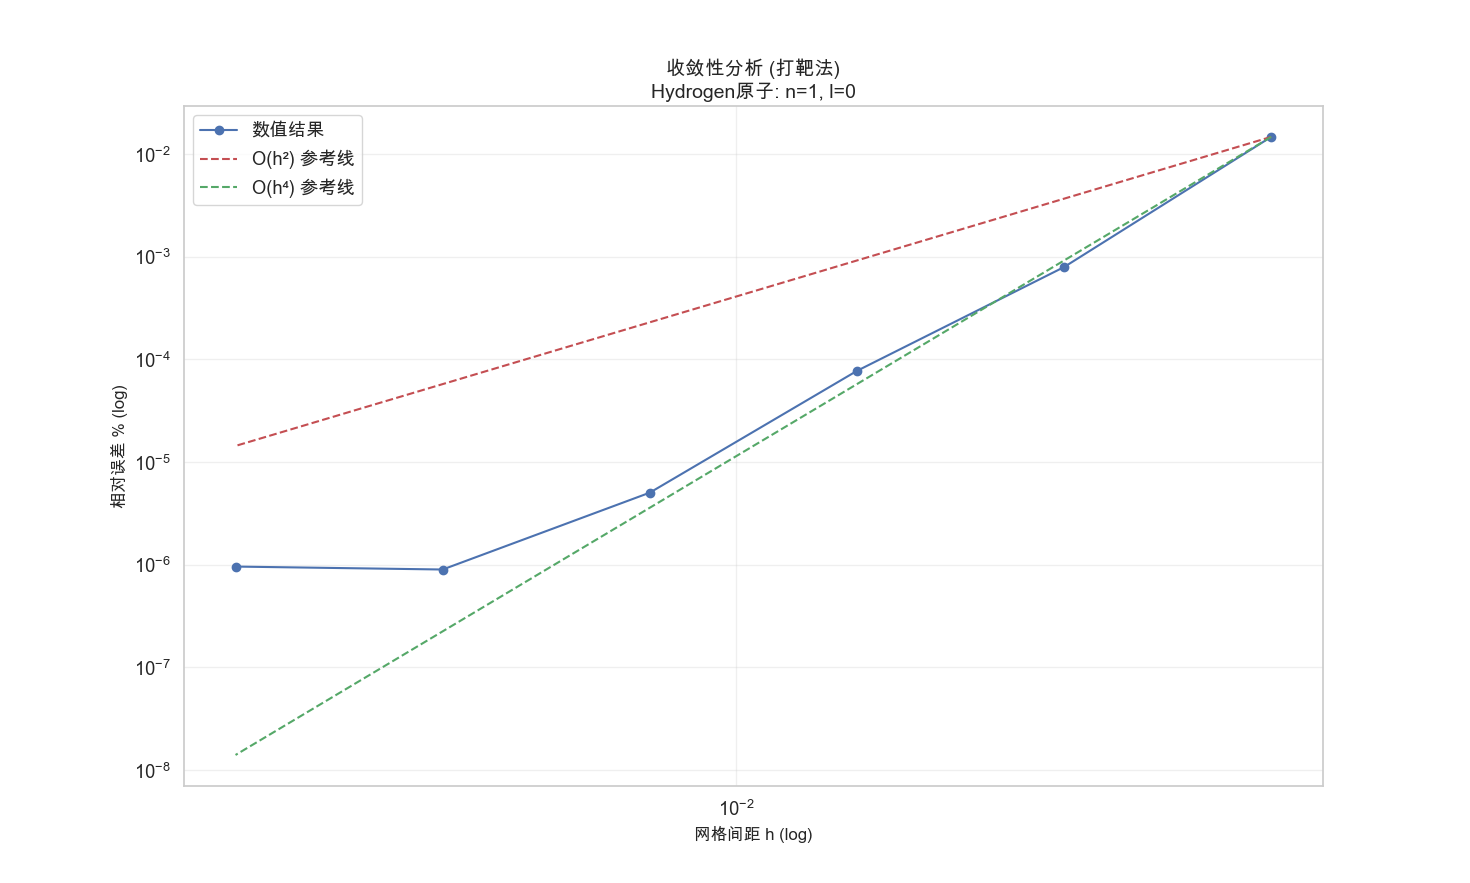
\includegraphics[width=1.0\textwidth]{Problem_2/figs/example_h_shooting_1s_con.png}
    \caption{使用打靶法求解氢原子库仑势的1s态的收敛性分析,验证了RK4全局误差是四阶精度的}
\end{figure}

\begin{figure}[H]
    \centering
    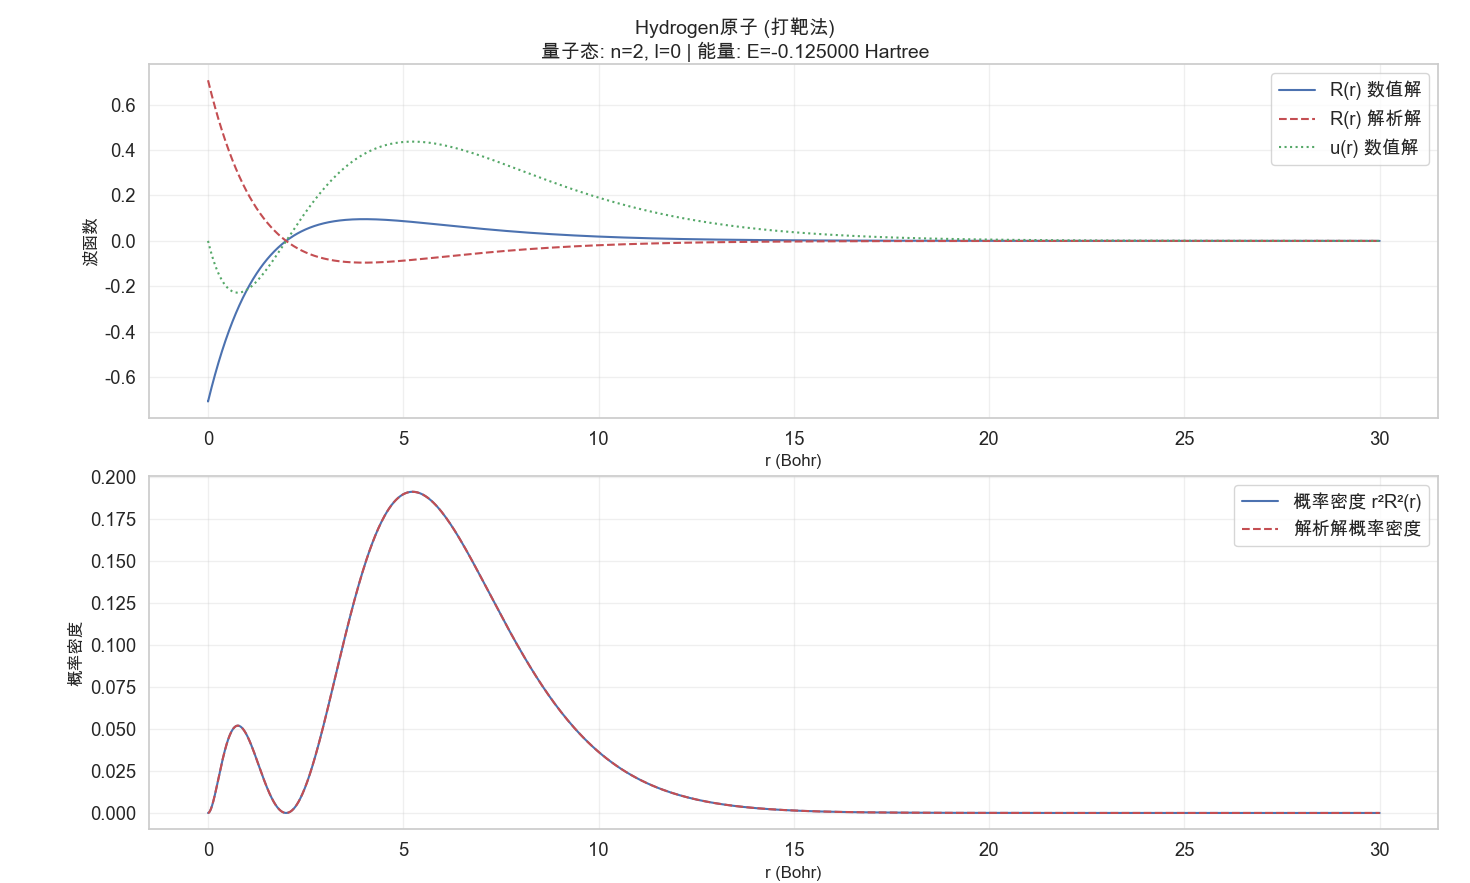
\includegraphics[width=1.0\textwidth]{Problem_2/figs/example_h_shooting_2s.png}
    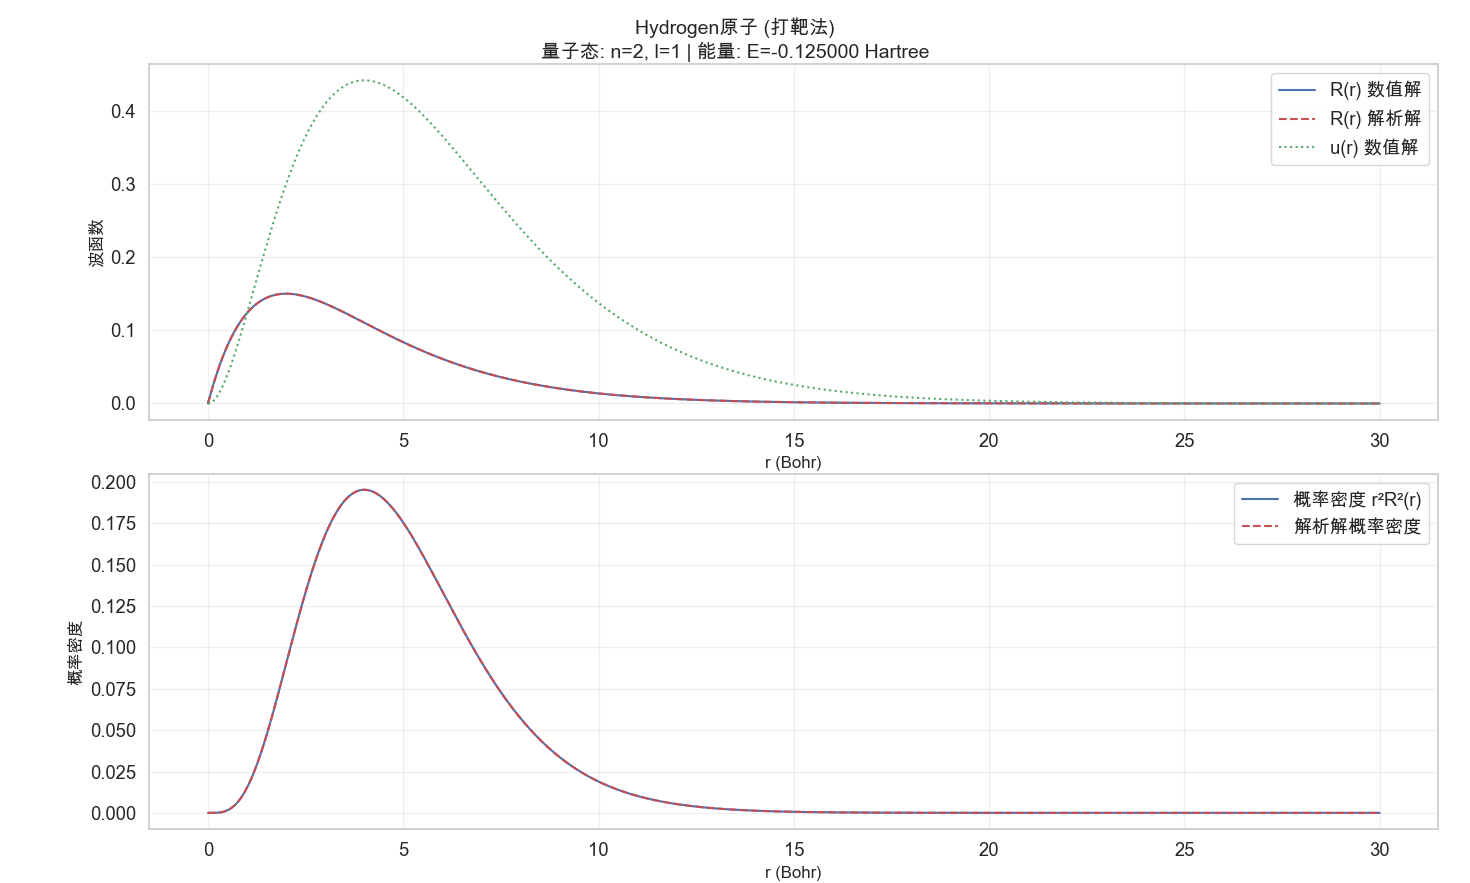
\includegraphics[width=1.0\textwidth]{Problem_2/figs/example_h_shooting_2p.png}
    \caption{使用打靶法求解氢原子库仑势的2s,2p态}
\end{figure}

\begin{figure}[H]
    \centering
    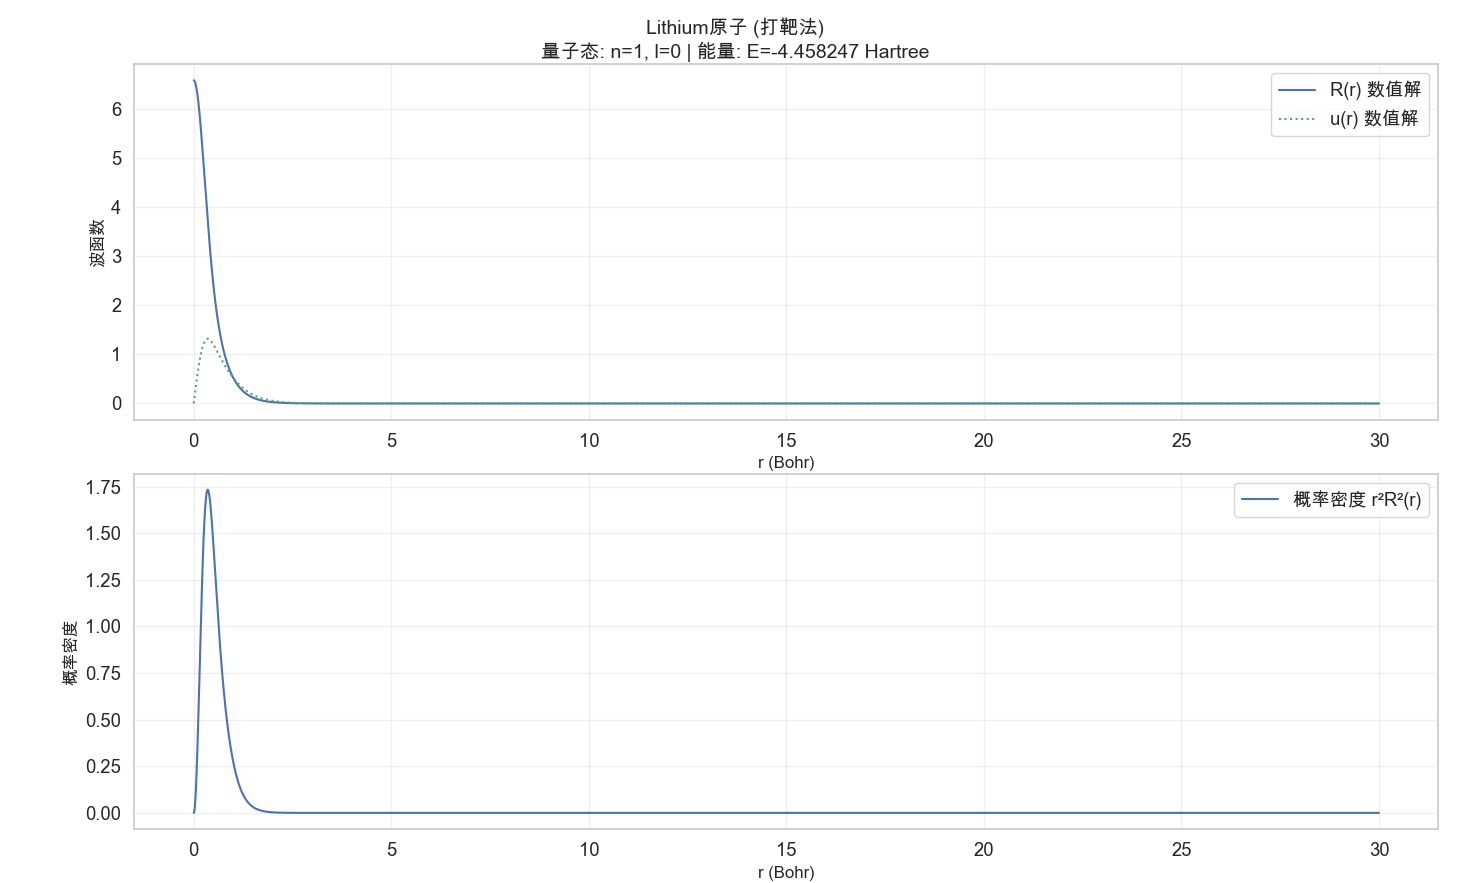
\includegraphics[width=1.0\textwidth]{Problem_2/figs/example_li_shooting_1s.png}
    \caption{使用打靶法求解锂原子局域势的1s态}
\end{figure}

\begin{figure}[H]
    \centering
    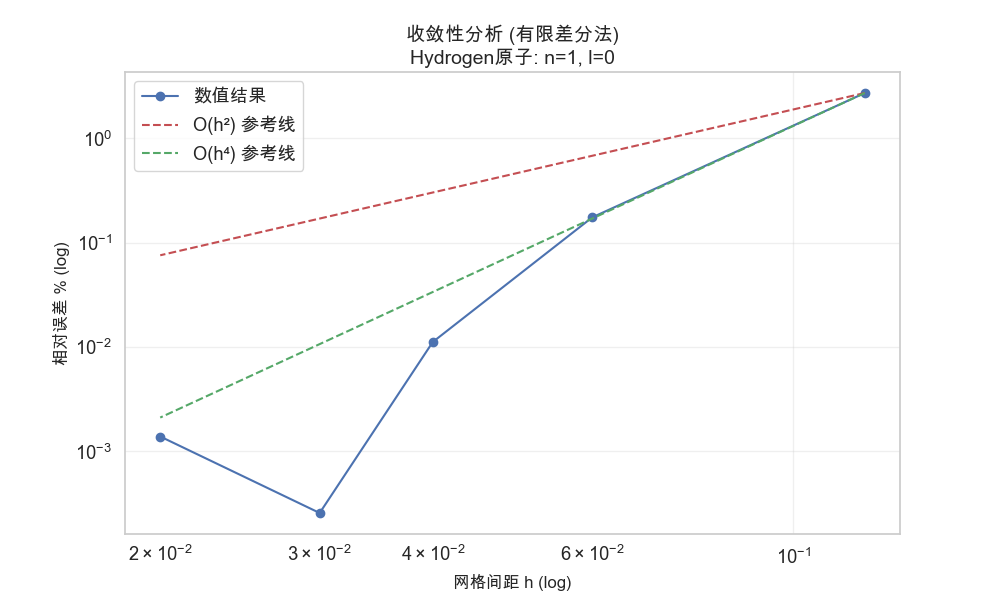
\includegraphics[width=0.8\textwidth]{Problem_2/figs/example_h_fd_1s_con.png}
    \caption{使用有限差分法求解氢原子库仑势的1s态的收敛性分析,新版本非均匀细网格的数值稳定性有所下降}
\end{figure}

\subsubsection{氢原子其它示例}
\begin{figure}[H]
    \centering
    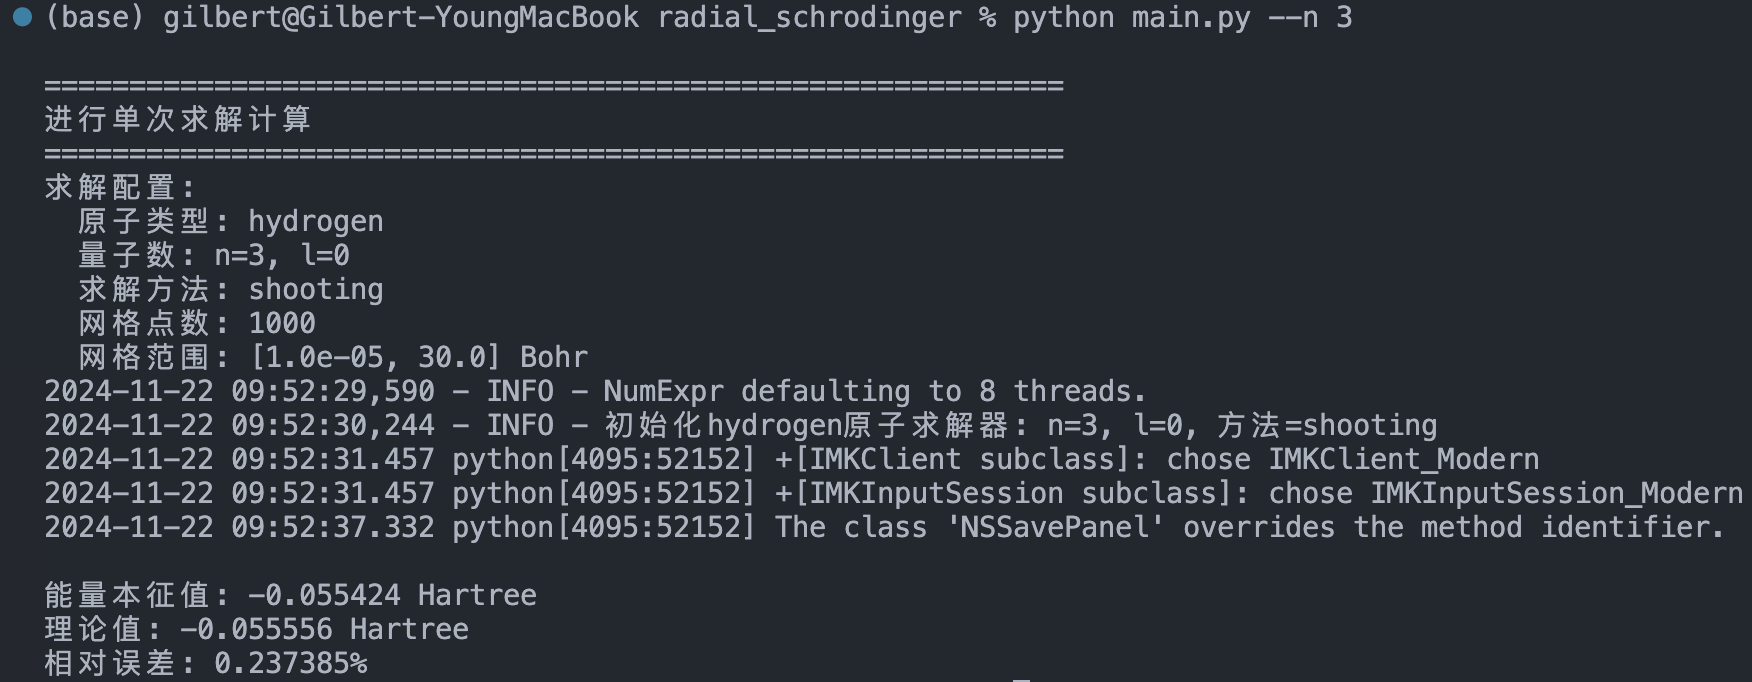
\includegraphics[width=1.0\textwidth]{Problem_2/figs/h_shooting_3s_terminal.png}
    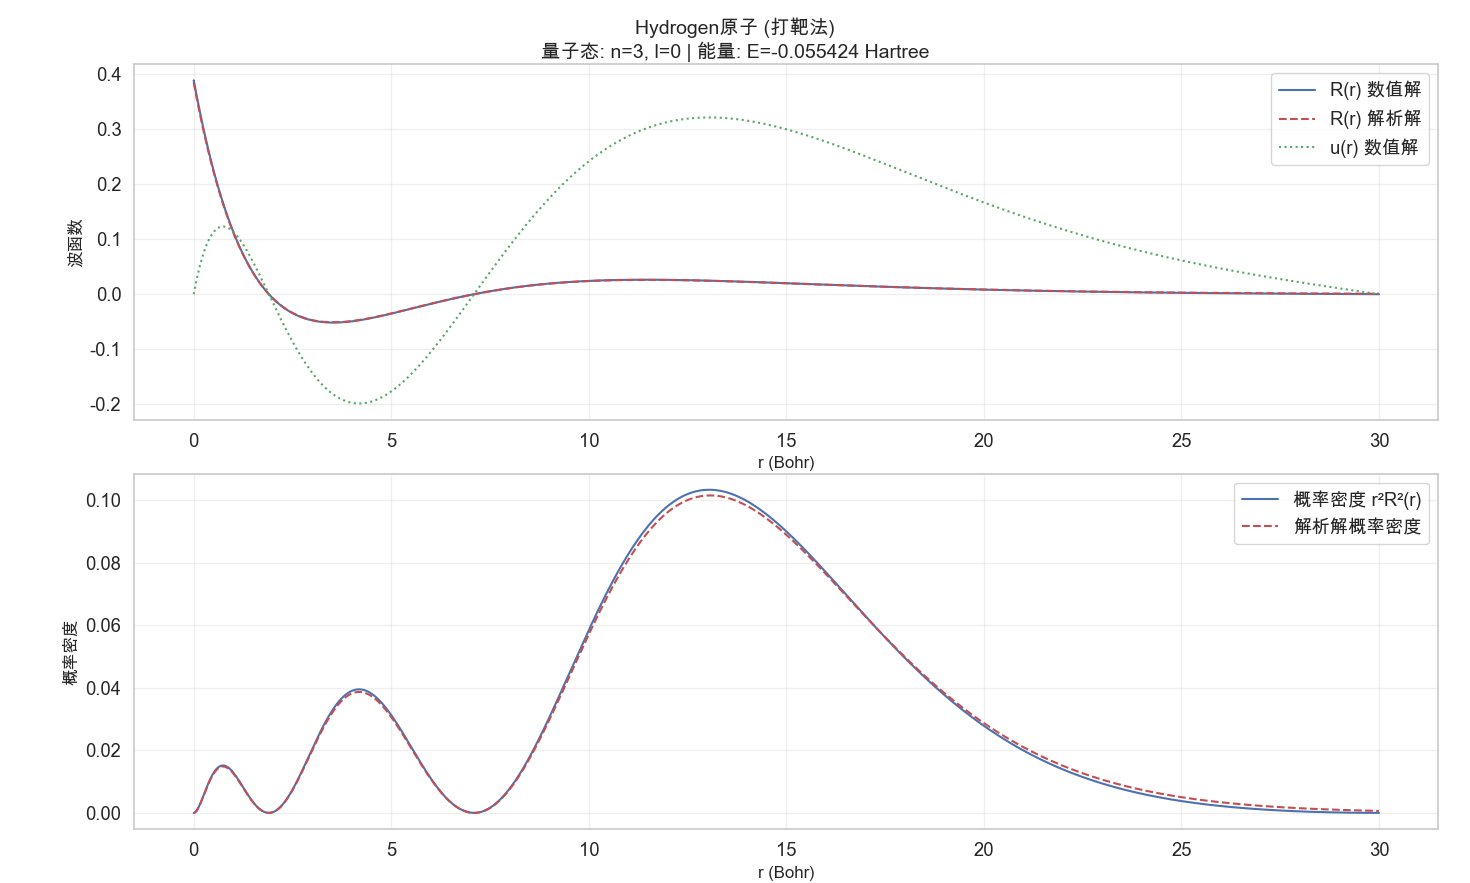
\includegraphics[width=1.0\textwidth]{Problem_2/figs/h_shooting_3s.png}
    \caption{使用打靶法求解氢原子库仑势的3s态,\texttt{r\_Max=30}的选项已经有些捉襟见肘}
\end{figure}

\begin{figure}[H]
    \centering
    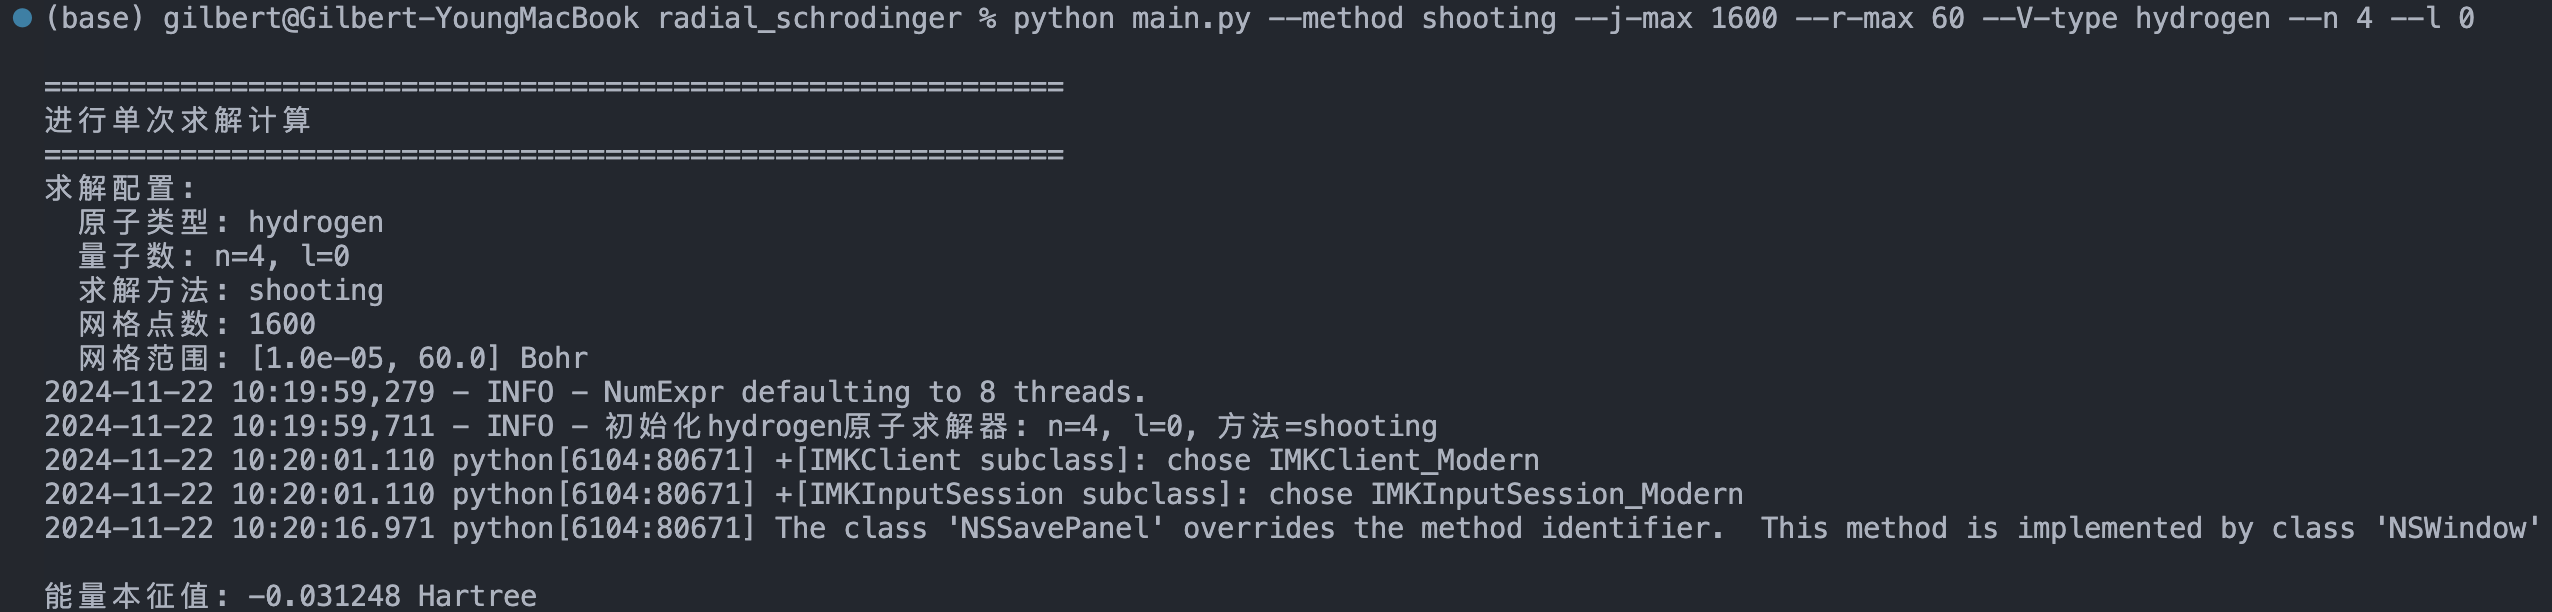
\includegraphics[width=0.6\textwidth]{Problem_2/figs/h_shooting_4s_terminal.png}
    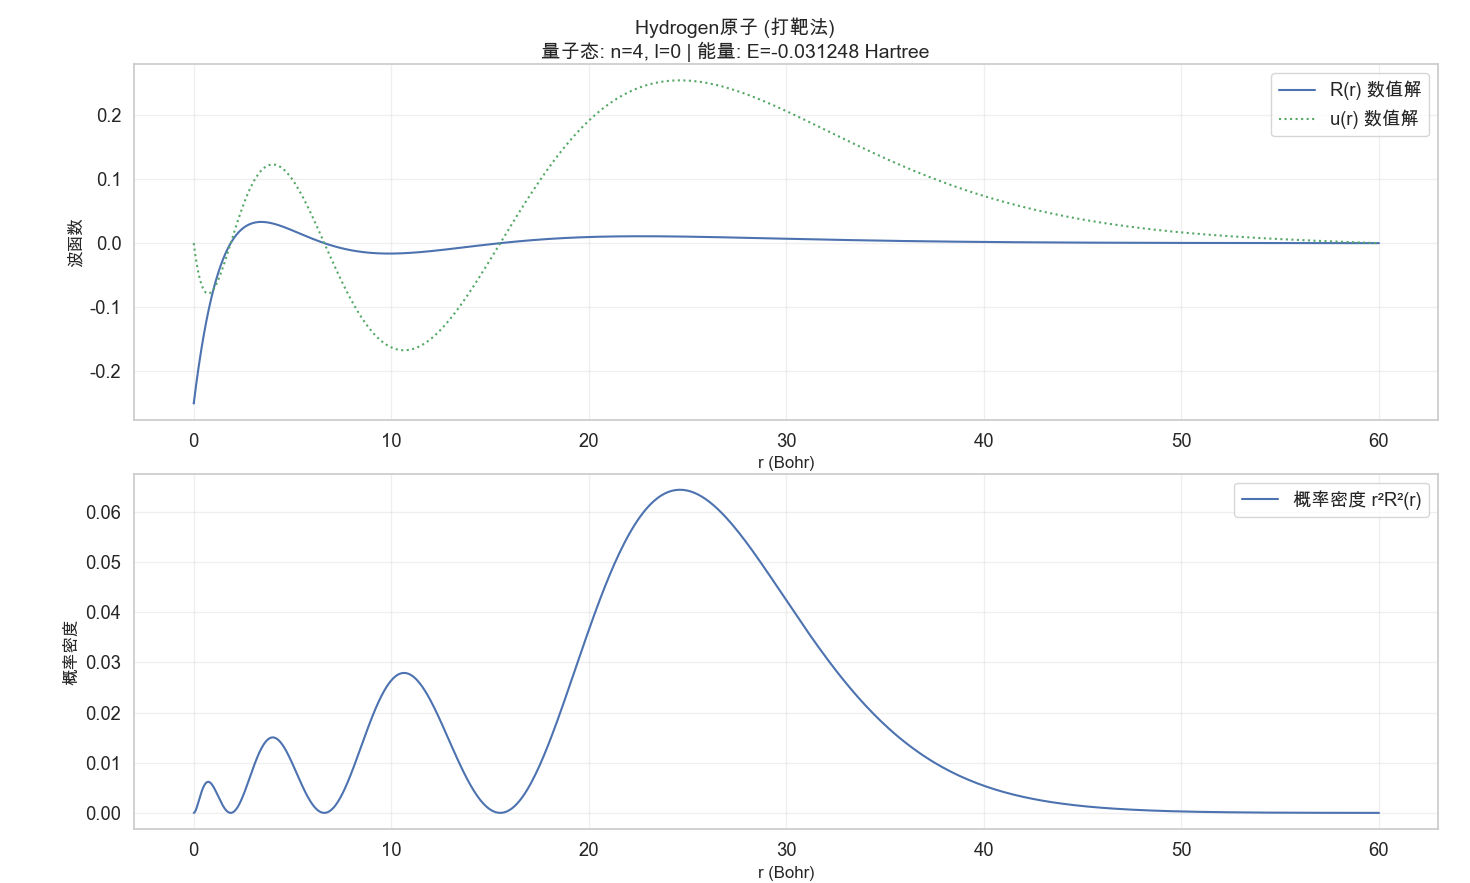
\includegraphics[width=0.6\textwidth]{Problem_2/figs/h_shooting_4s.png}
    \caption{使用打靶法求解氢原子库仑势的4s态,指定\texttt{r\_Max=60}}
\end{figure}

\begin{figure}[H]
    \centering
    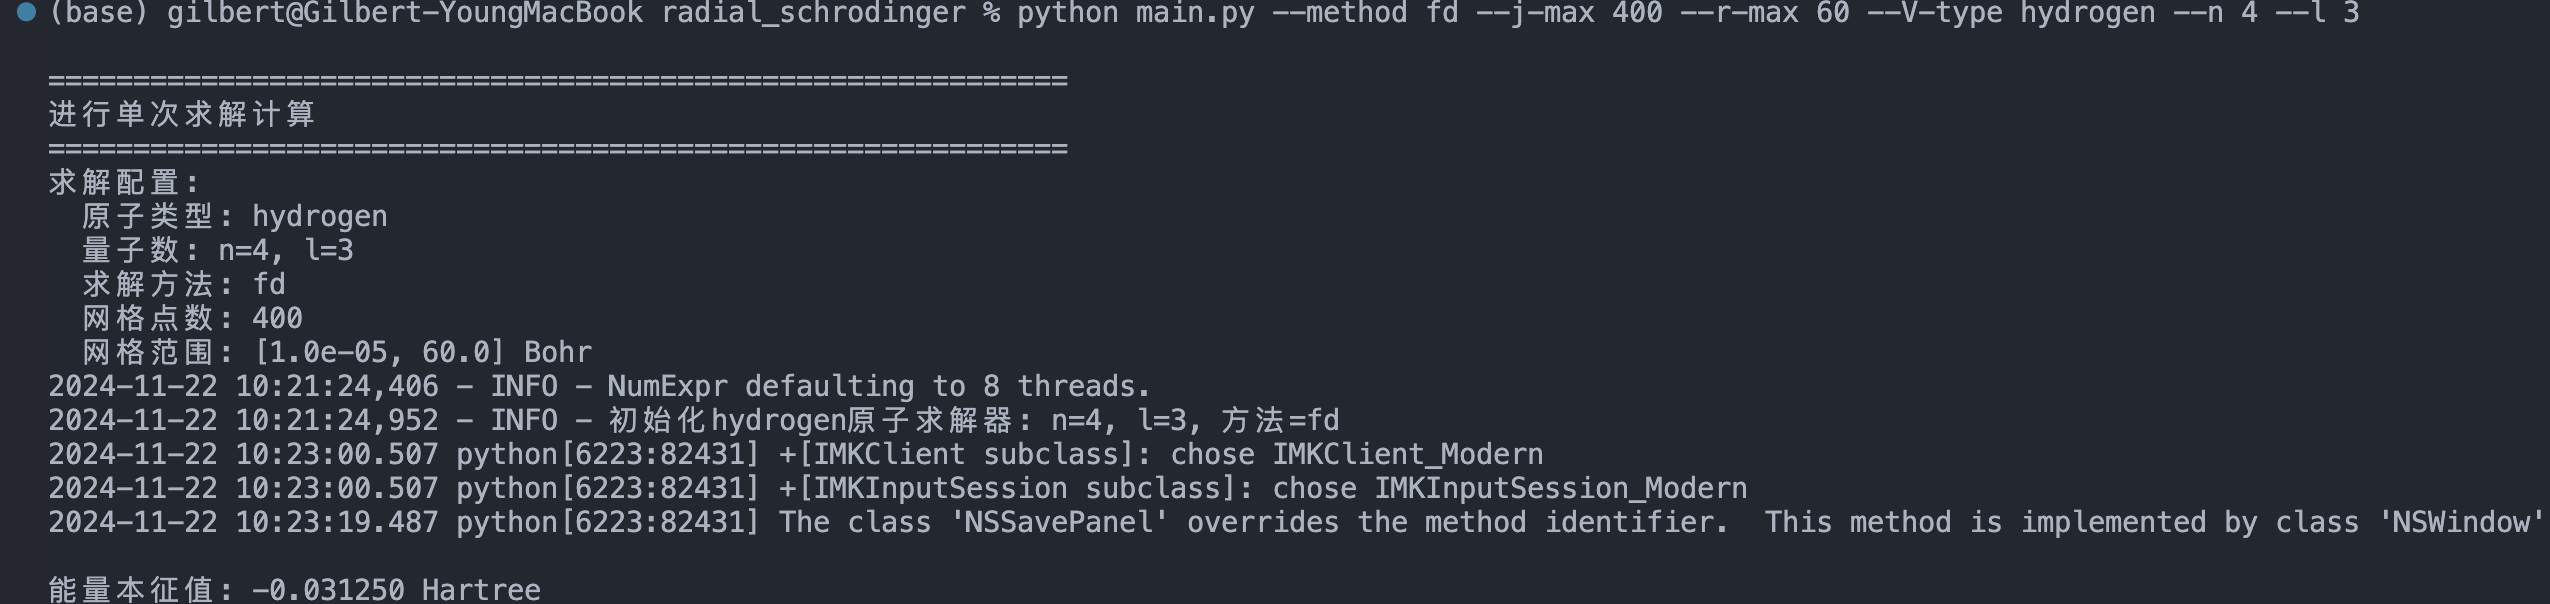
\includegraphics[width=0.6\textwidth]{Problem_2/figs/h_fd_4f_terminal.png}
    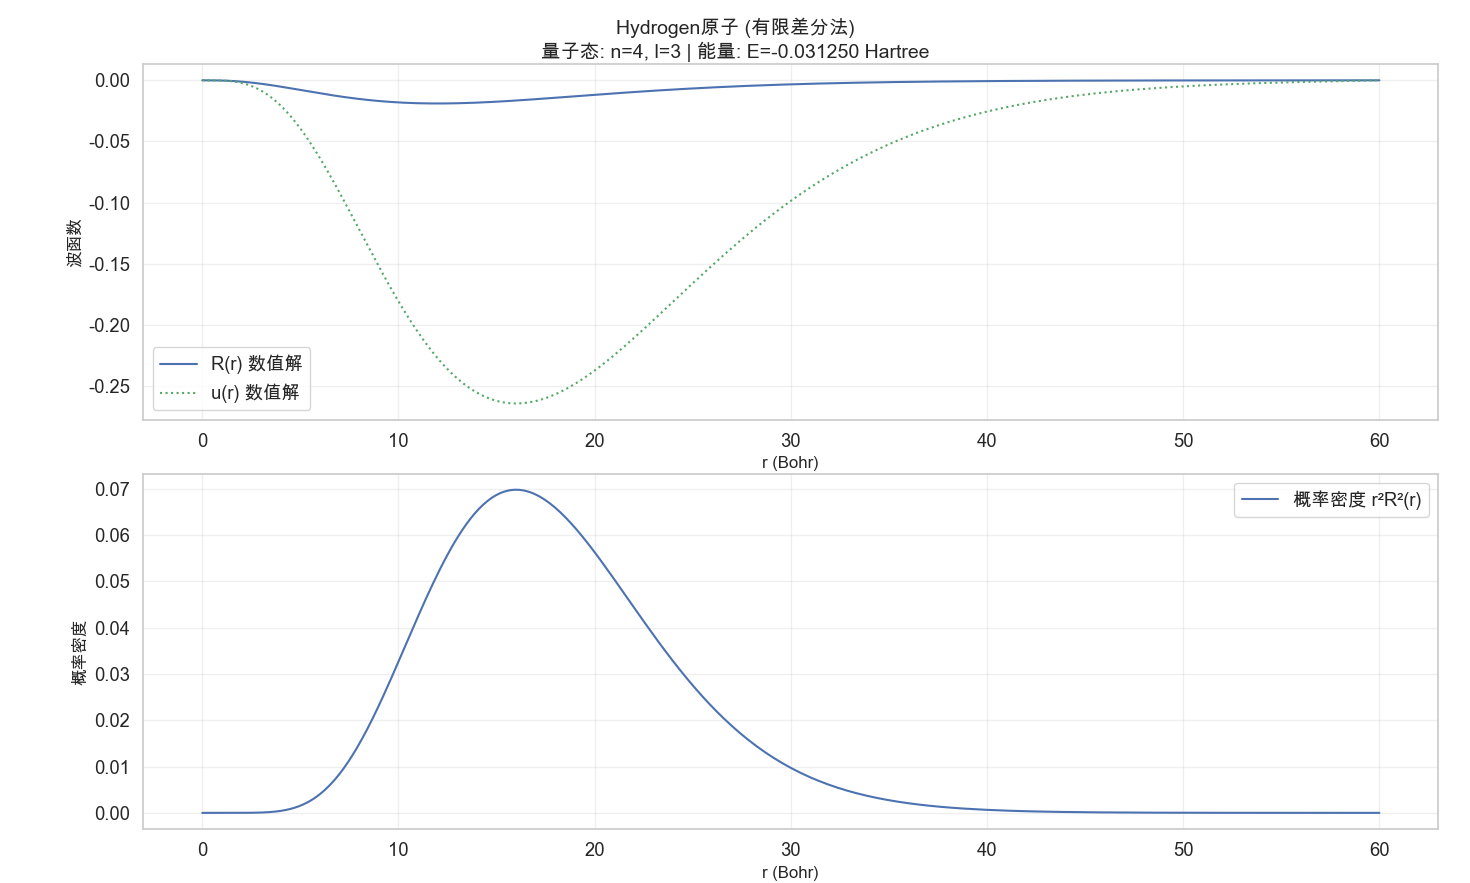
\includegraphics[width=0.6\textwidth]{Problem_2/figs/h_fd_4f.png}
    \caption{使用有限差分法求解氢原子库仑势的4f态,指定\texttt{r\_Max=60}}
\end{figure}

\subsubsection{锂原子其它示例}
\begin{figure}[H]
    \centering
    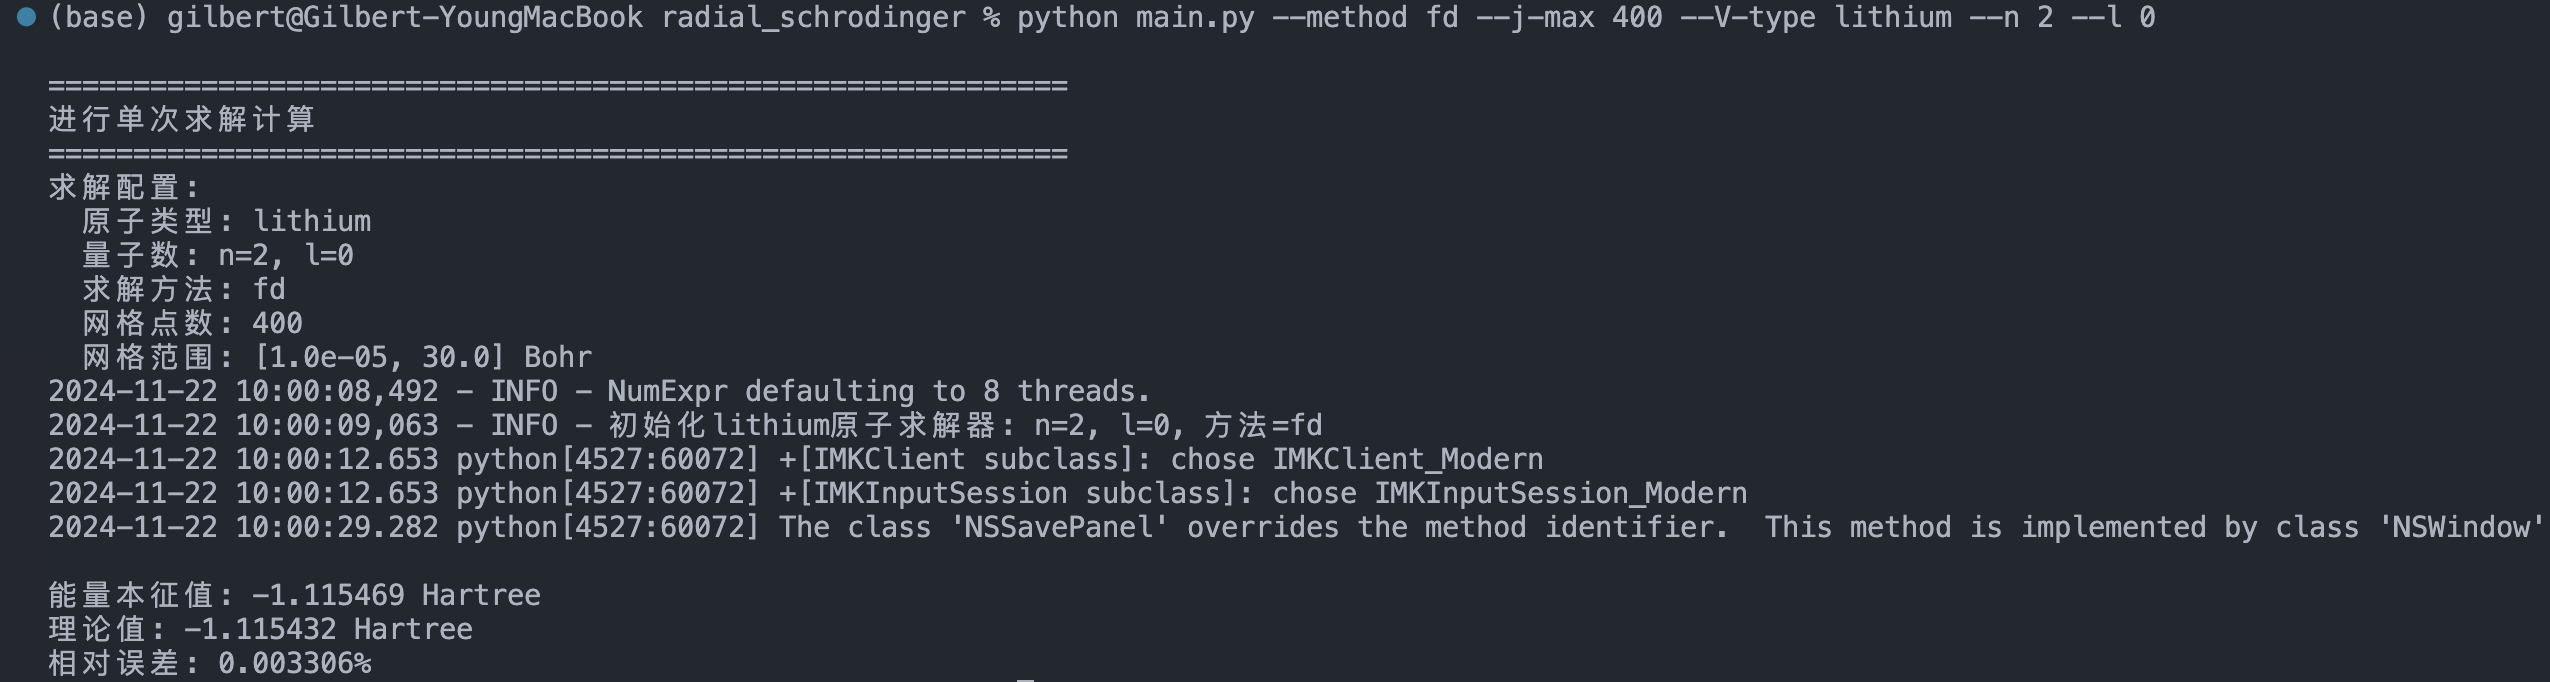
\includegraphics[width=0.6\textwidth]{Problem_2/figs/li_fd_2s_terminal.png}
    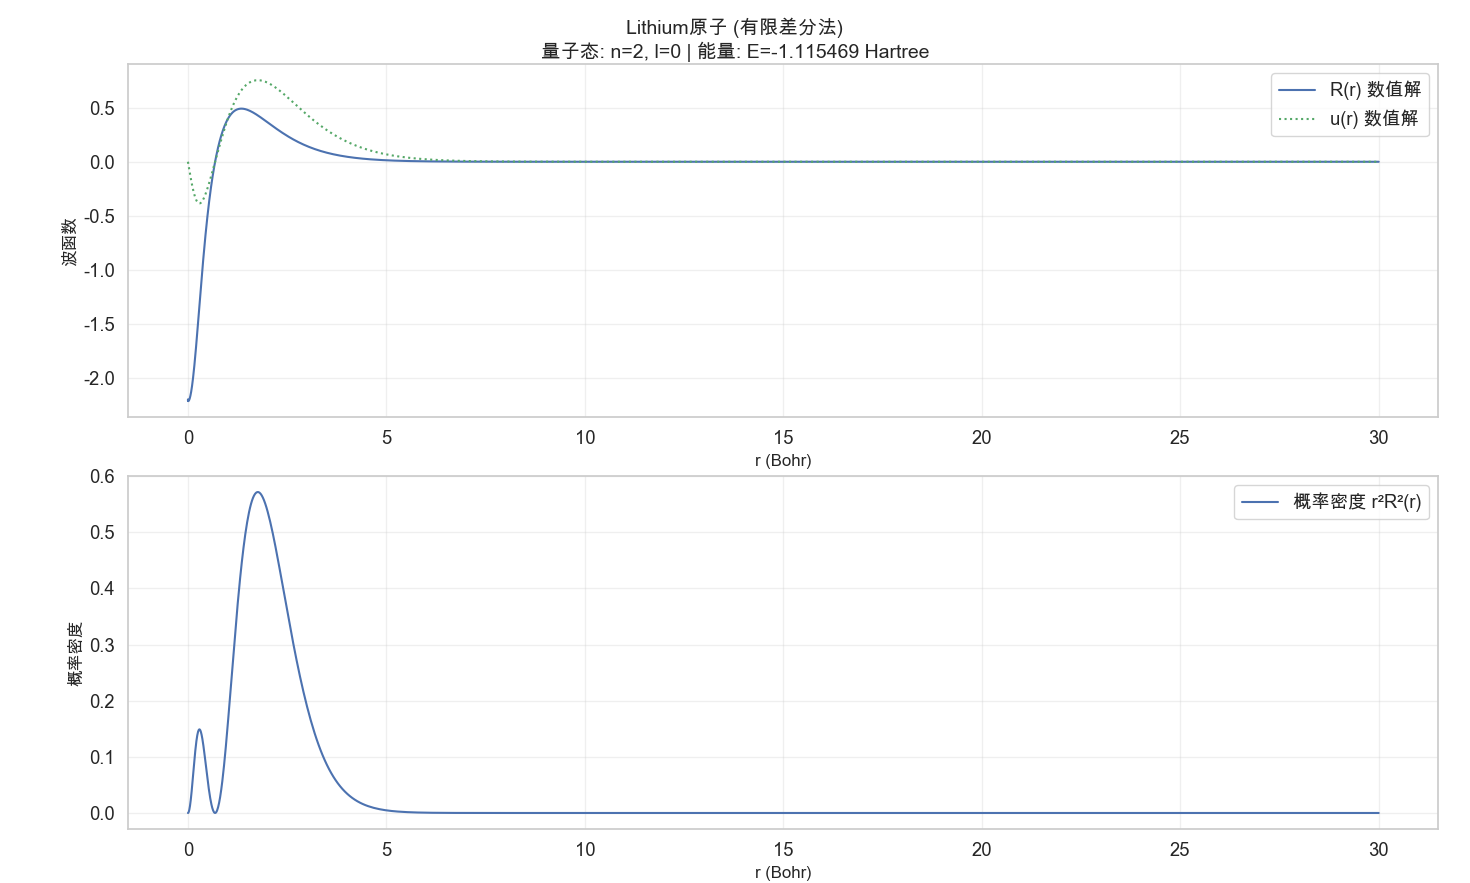
\includegraphics[width=0.6\textwidth]{Problem_2/figs/li_fd_2s.png}
    \caption{使用有限差分法求解锂原子局域势的2s态}
\end{figure}

\begin{figure}[H]
    \centering
    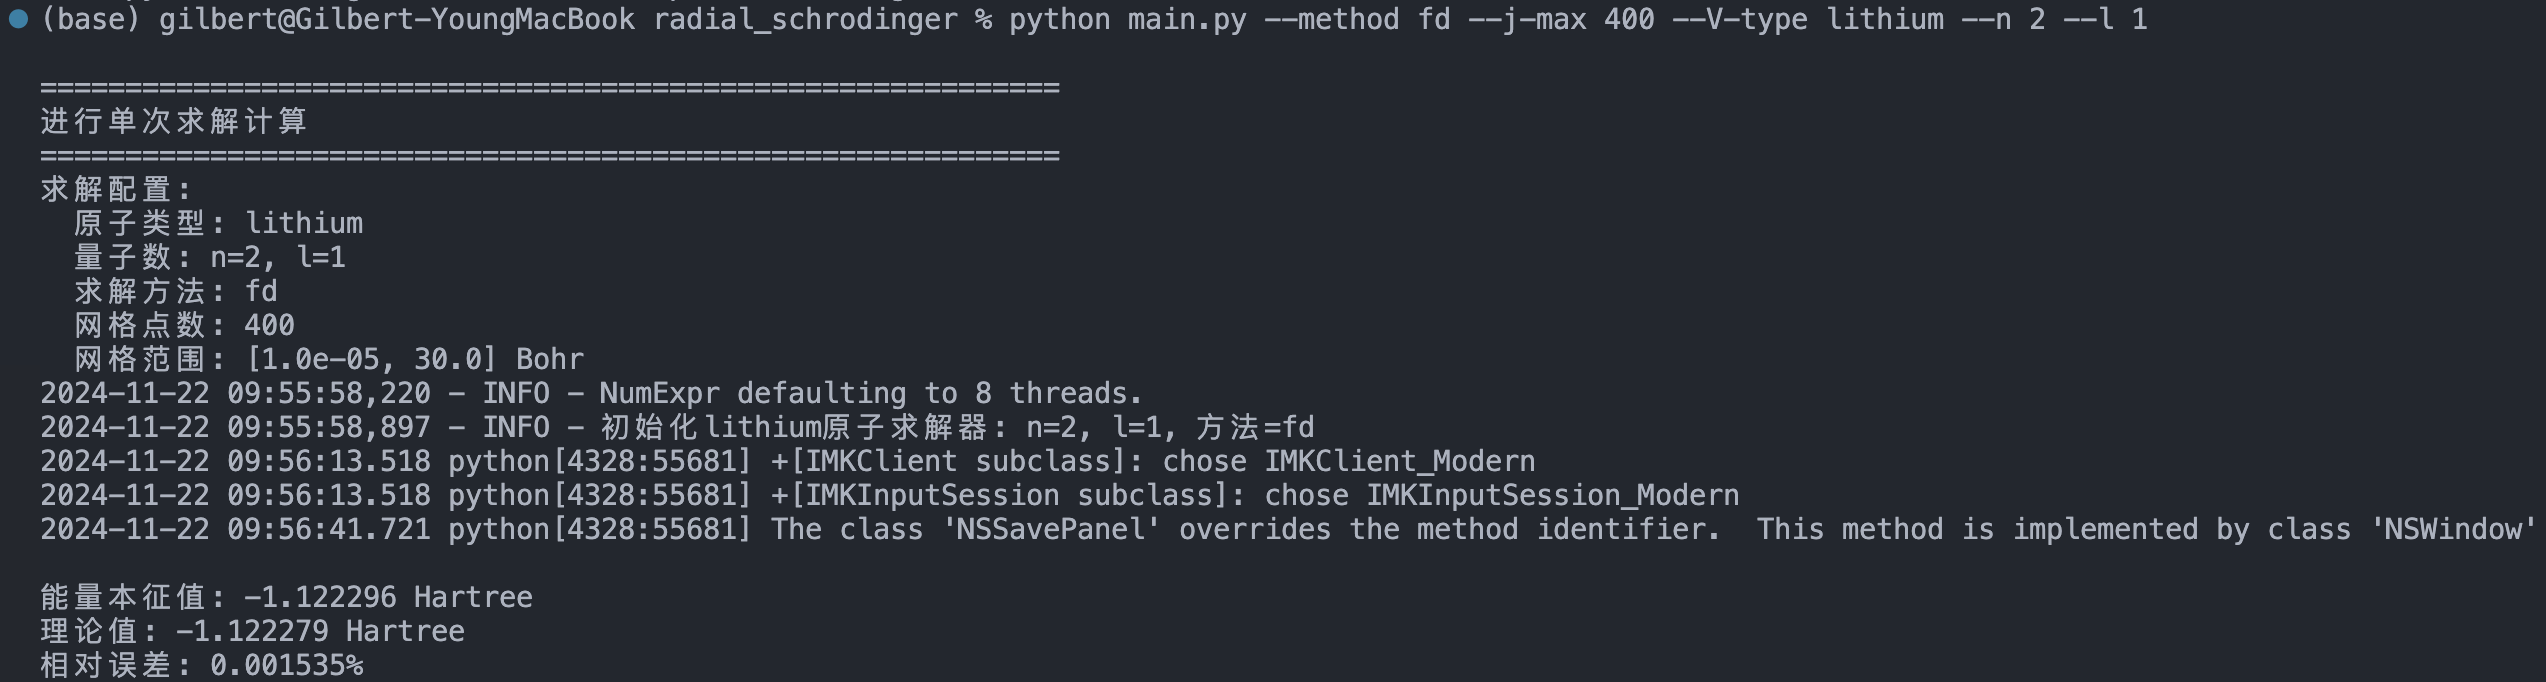
\includegraphics[width=0.6\textwidth]{Problem_2/figs/li_fd_2p_terminal.png}
    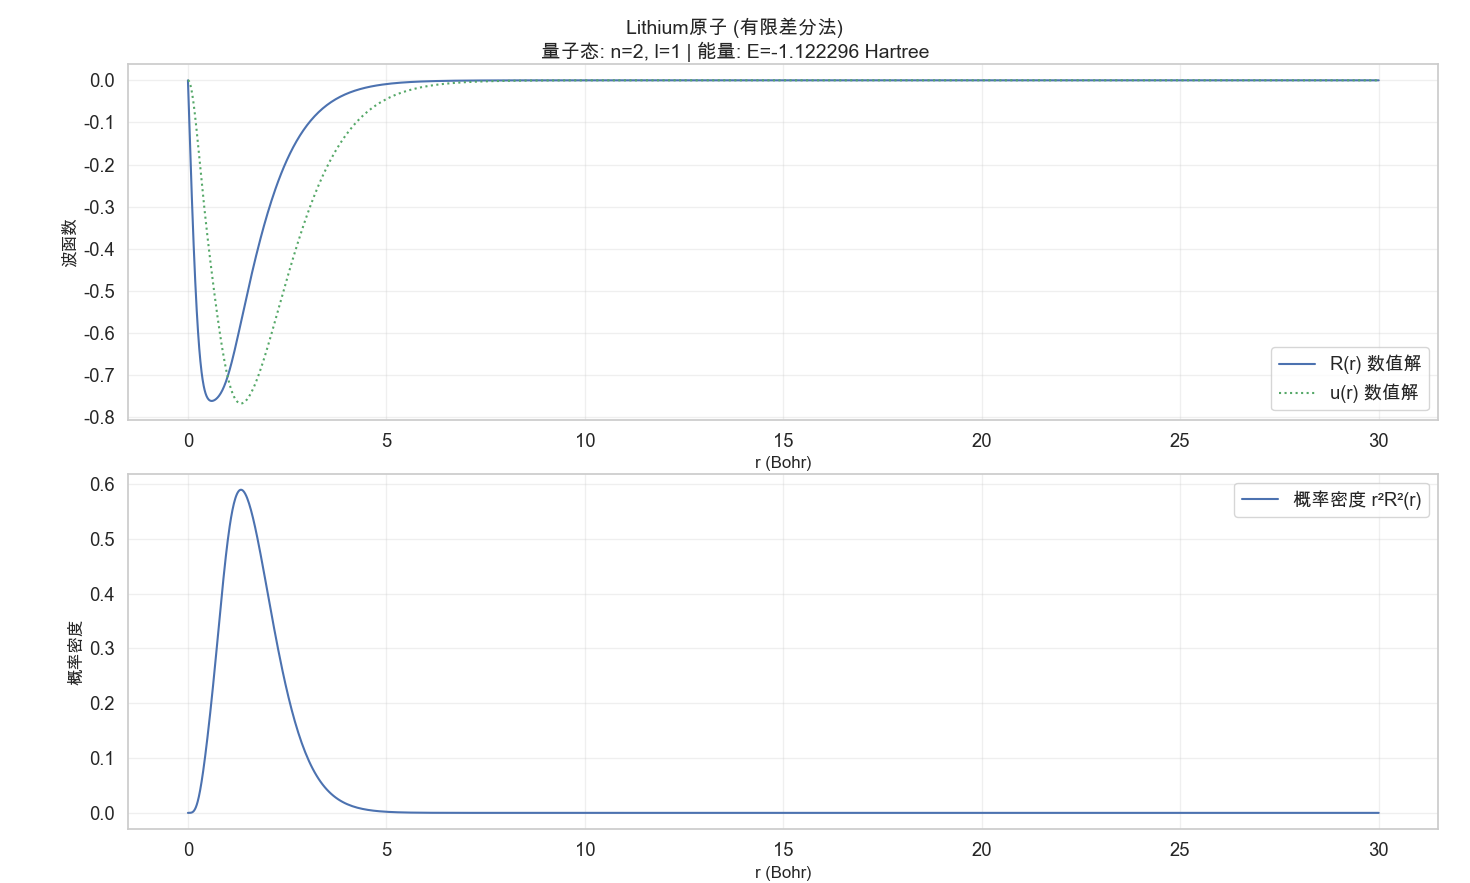
\includegraphics[width=0.6\textwidth]{Problem_2/figs/li_fd_2p.png}
    \caption{使用有限差分法求解锂原子局域势的2p态}
\end{figure}

\begin{figure}[H]
    \centering
    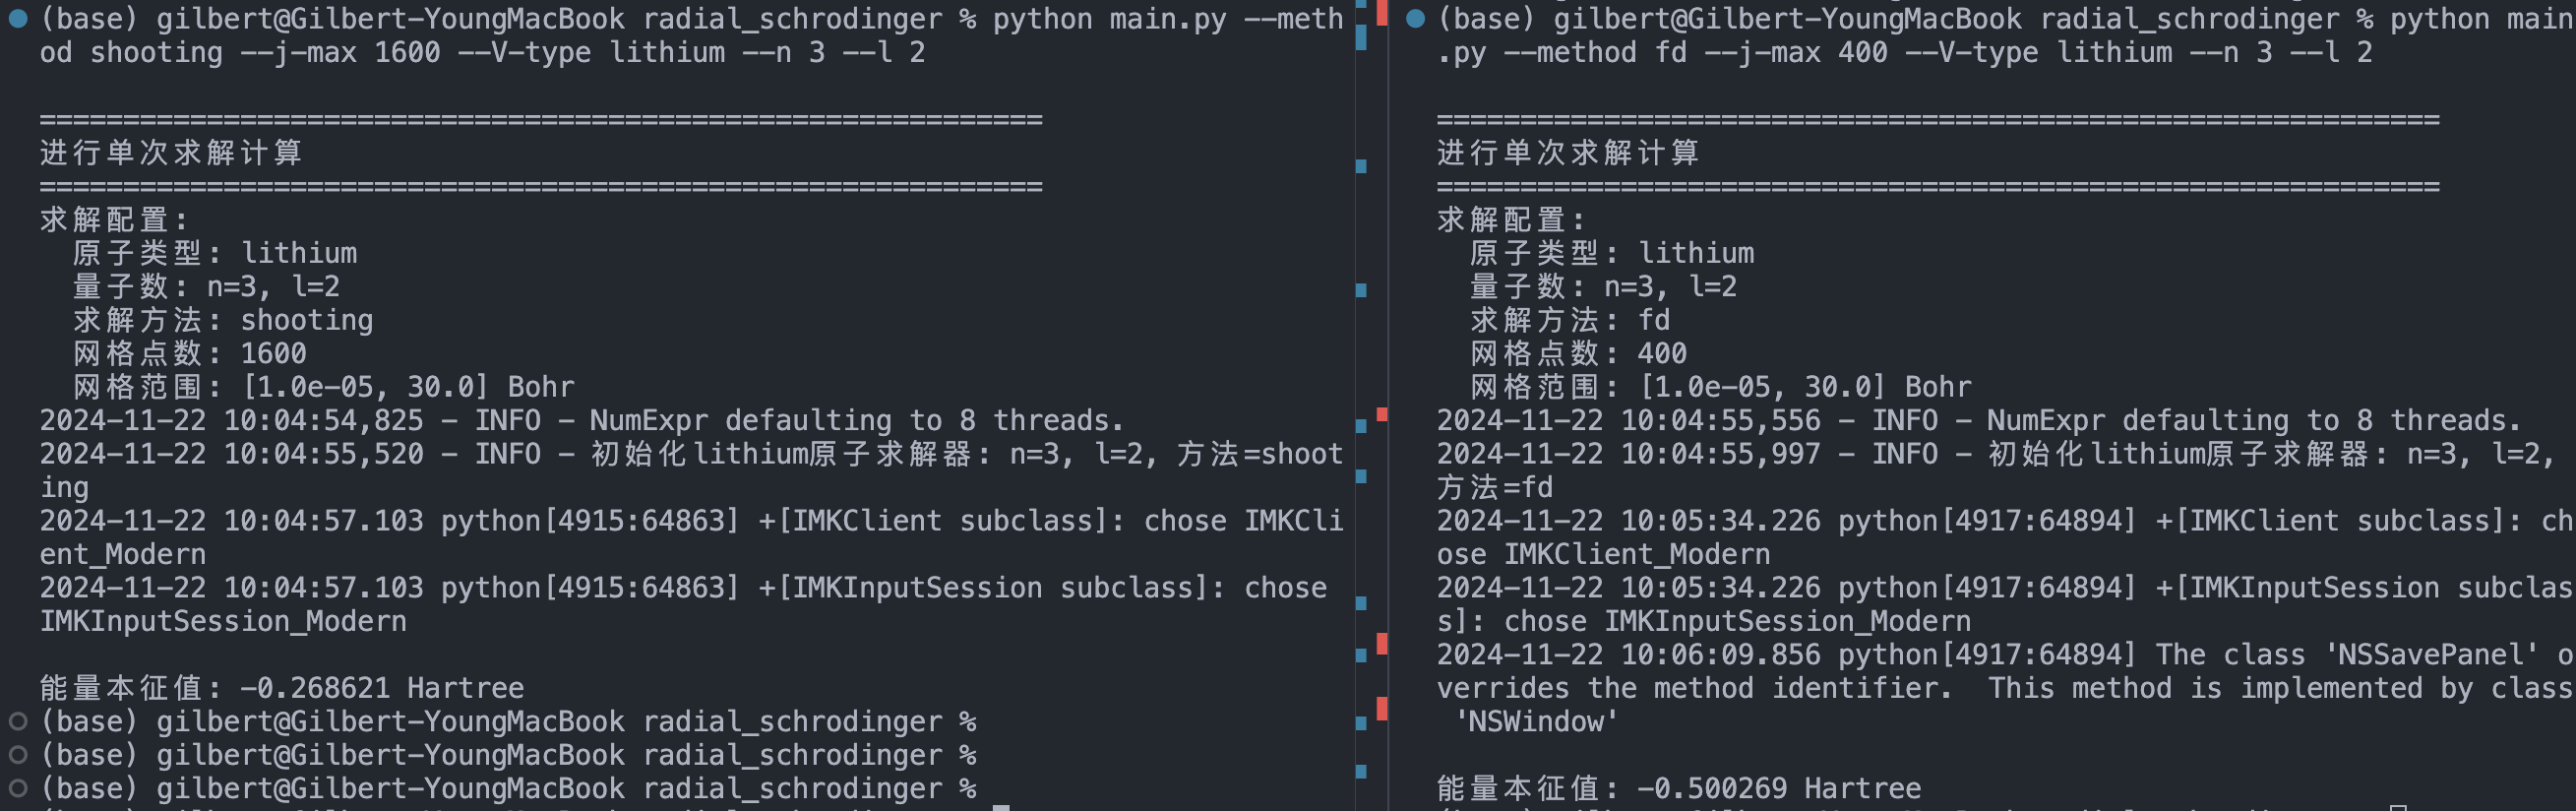
\includegraphics[width=0.8\textwidth]{Problem_2/figs/li_sh&fd_3d_terminal.png}
    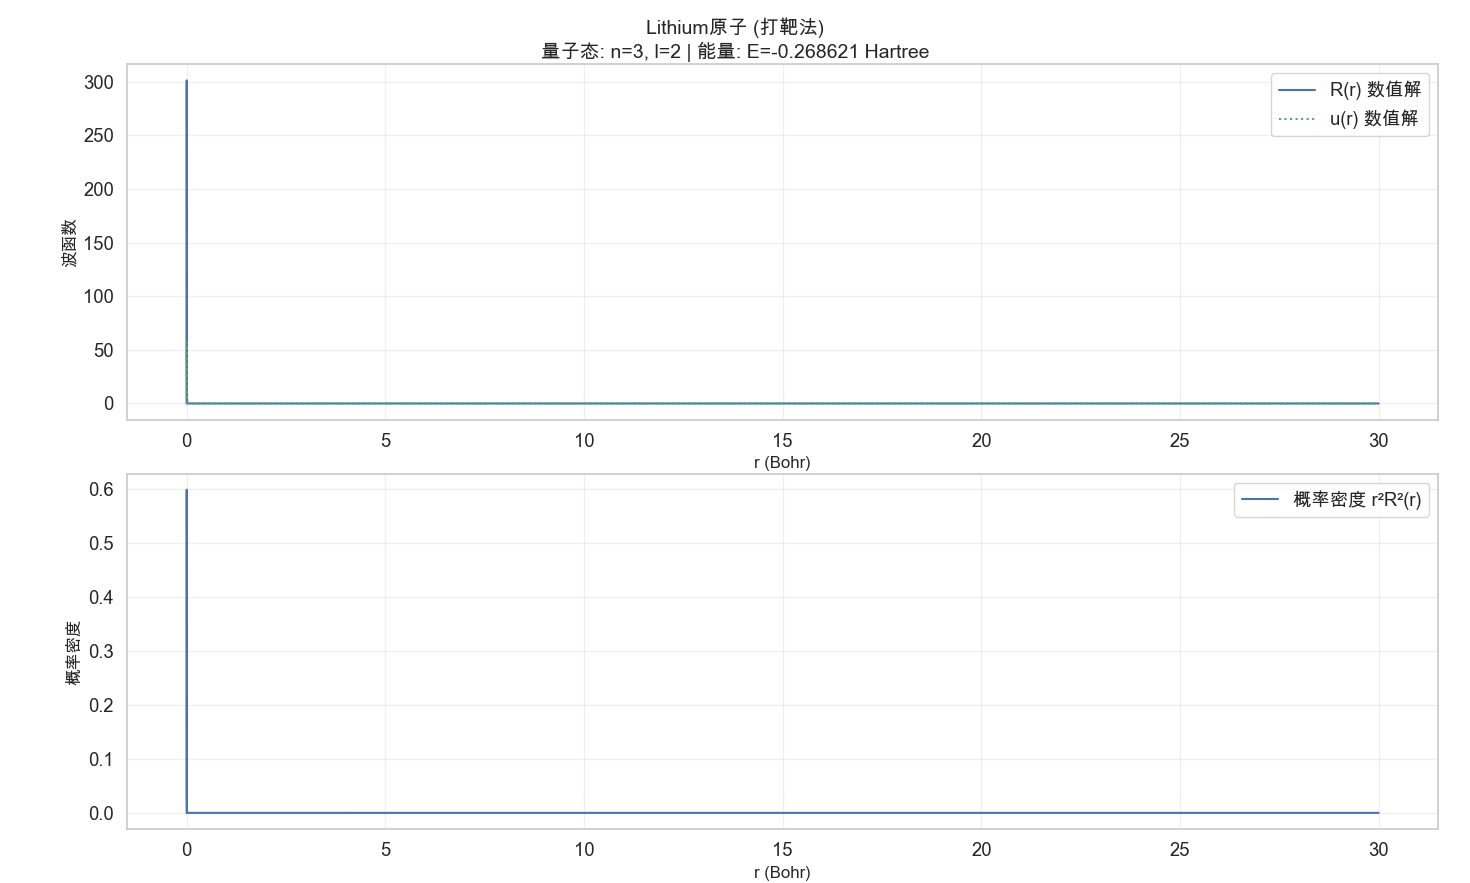
\includegraphics[width=0.8\textwidth]{Problem_2/figs/li_shooting_3d.png}
    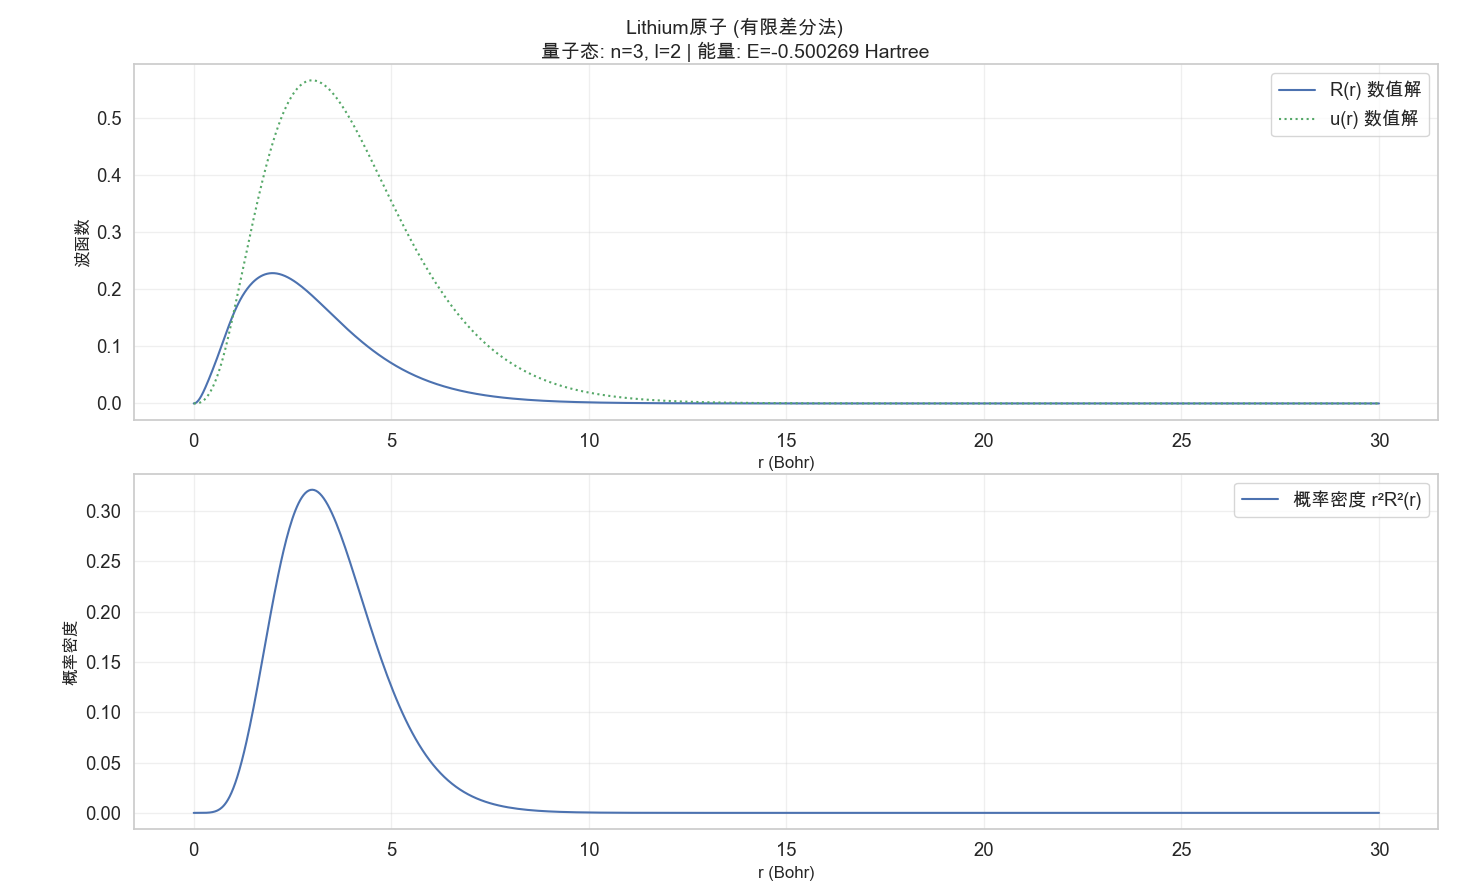
\includegraphics[width=0.8\textwidth]{Problem_2/figs/li_fd_3d.png}
    \caption{分别使用打靶法与有限差分法求解锂原子局域势的3d态,其中打靶法必须拓展\texttt{r\_Max},否则无法收敛}
\end{figure}
